\PassOptionsToPackage{unicode,bookmarks=true}{hyperref}
\documentclass{beamer}
%
% Choose how your presentation looks.
%
% For more themes, color themes and font themes, see:
% http://deic.uab.es/~iblanes/beamer_gallery/index_by_theme.html
%
\mode<presentation>
{
  \usetheme{Copenhagen}      % or try Darmstadt, Madrid, Warsaw, ...
  \usecolortheme{seagull} % or try albatross, beaver, crane, ...
  \usefonttheme{default}  % or try serif, structurebold, ...
  \setbeamertemplate{navigation symbols}{}
  \setbeamertemplate{caption}[numbered]
  \setbeamertemplate{bibliography item}{}
} 

\usepackage{etoolbox}
\makeatletter
\newcommand{\dontusepackage}[2][]{%
  \csdef{ver@#2.sty}{9999/12/31}%
  \csdef{opt@#2.sty}{#1}}
\newcommand{\pretendpackagewasnotloaded}[1]{%
  \csundef{ver@#1.sty}%
  \csundef{opt@#1.sty}}
\makeatother

\usepackage{array, booktabs}
\usepackage[utf8]{inputenc}
\usepackage[T2A]{fontenc} % enable Cyrillic fonts
\dontusepackage{ucs}
\usepackage[english,serbianc]{babel}
\pretendpackagewasnotloaded{ucs}
\usepackage[backend=biber, bibstyle=nature, sorting=nty, citestyle=numeric-comp]{biblatex}
\addbibresource{literatura.bib}


\title[Генетичко програмирање]{Генетичко програмирање}
\author[Стојановић, Ивановић, Стефановић, Поповић]{Александра Стојановић, Ивана Ивановић,\linebreak Александар Стефановић, Оливера Поповић}
\institute[МАТФ]{Математички факултет\\Универзитет у Београду}
\date{21. април 2020.}

\graphicspath{ {./Images/} }
\setcounter{tocdepth}{1}

\begin{document}

\begin{frame}
  \titlepage
\end{frame}

% Uncomment these lines for an automatically generated outline.
\begin{frame}{Садржај}
  \tableofcontents
\end{frame}

\section{Историјат}

\begin{frame}{Историјат}
    \begin{itemize}
        \item 1948 — Алан Тјуринг
        \item 1962 — Џон Холанд
        \item Представљање бројева низовима битова фиксне дужине у проблемима оптимизације
        \item Холанд и Раитман — Систем класификатора
        \item Смит — Репрезентација променљиве дужине
        \item 1981 — Форсит — Репрезентација помоћу стабала
        \item 1985 — Крамер
    \end{itemize}
\end{frame}

\begin{frame}{Историјат}
    \begin{itemize}
        \item Џон Коза
        \begin{itemize}
            \item 1989 — документовање методе која је користила универзални језик
            \item 1992 — објављивање књиге
            \item 1996 — годишња конференција о ГП-у
            \item 1998 — први уџбеник ГП-а
        \end{itemize}
        \item Рик Риоло — наставак процвата ГП-а
        \item 2003 — годишња радионица
    \end{itemize}
\end{frame}

\section{Опис алгоритма}

\begin{frame}{Опис алгоритма}
    \begin{itemize}
        \item Инспирисан процесом еволуције у природи
        \item Спада у групу алгоритама \textbf{еволутивног  израчунавања}	
        \item Процес природне селекције
        \item Комбиновање гена
    \end{itemize}
    \begin{center}
        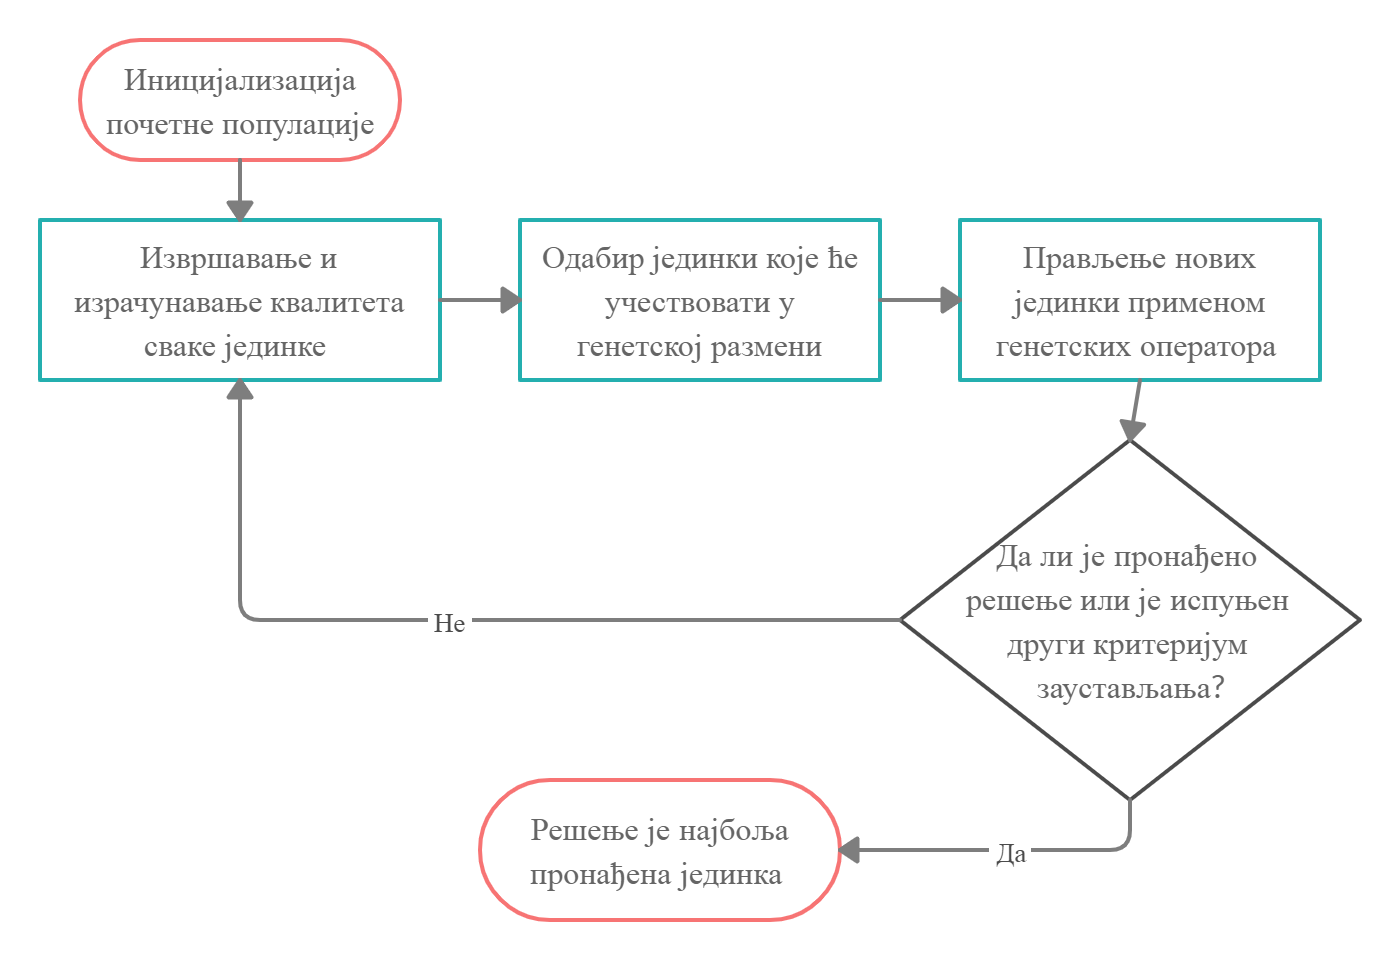
\includegraphics[scale=0.14]{opsti_algoritam.png}
    \end{center}
\end{frame}
    
\subsection[Репрезентација јединки]{Репрезентација јединки}

\begin{frame}{Опис алгоритма}
    \begin{itemize}
        \item јединке — рачунарски програми
        \item синтакснo стаблo — примитивни скуп ГП-а
        \begin{itemize}
            \item терминали — променљиве и константе — листови
            \item функције — аритметичке, логичке... — остали чворови
        \end{itemize}
    \end{itemize}
    \begin{minipage}{0.6\textwidth}
        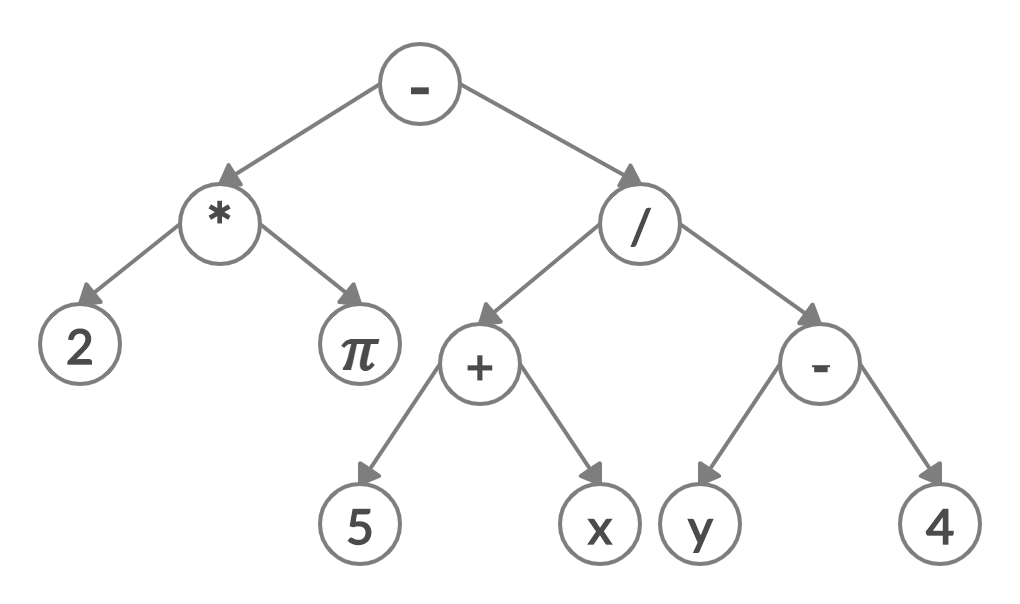
\includegraphics[scale=0.18]{sintaksno_stablo.png}
    \end{minipage}
    \begin{minipage}{0.35\textwidth}\raggedleft
        \begin{equation*} 
            2*\pi-\frac{5+x}{y-4}
        \end{equation*}
        \begin{center}
        скуп терминала:\\
        \{2, $\pi$, 5, x, y, 4\}\\
        скуп функција:\\
        \{+, -, *, /\}
        \end{center}
    \end{minipage}
\end{frame}
    
\subsection[Иницијализација популације и функција прилагођености]{Иницијализација популације и функција прилагођености}

\begin{frame}{Опис алгоритма}
    \begin{itemize}
        \item Методе за генерисање почетне популације:
        \begin{itemize}
            \item потпуна метода (eng. full method)
            \item метода раста (eng. grow method)
            \item комбинована метода
        \end{itemize}
    \end{itemize}
    Функција прилагођености (eng. fitness function) даје оцену \textbf{квалитета јединке}.
    \begin{itemize}
        \item могућност израчунавања за сваку јединку
        \item ефикасност израчунавања
        \item мера квалитета јединке / додела пенала
    \end{itemize}
\end{frame}
    
\subsection[Селекција, репродукција и мутација]{Селекција, репродукција и мутација}

\begin{frame}{Опис алгоритма}
    Селекција — проналажење боље прилагођених јединки
    \begin{minipage}{0.5\textwidth}
        \begin{itemize}
            \item Турнирска селекција
            \item Рулетска селекција
        \end{itemize}
    \end{minipage}
    \begin{minipage}{0.45\textwidth}\raggedleft
        \begin{equation*}
            p_i = \frac{f(i)}{\sum_{j}^{N} f(i)}
        \end{equation*}
    \end{minipage}
    Репродукција — добијање потомства од два родитеља добијених селекцијом
    \begin{itemize}
        \item метод укрштања стабала
        \item бирање функција 90\% времена, а листова преосталих 10\% 
    \end{itemize}
    Мутација — јединке не буду превише сличне 
    \begin{itemize}
        \item избегавање локалног екстремума
        \item бирање тачке јединке на случајан начин:
        \begin{itemize}
            \item подстабло са кореном у тој тачки се мења случајно генерисаним стаблом
            \item вредност у том чвору се замени случајно одабраном вредошћу исте арности из примитивног скупа
        \end{itemize}
    \end{itemize}
\end{frame}

\subsection[Прилагођавање алгоритма]{Прилагођавање алгоритма}
    
\begin{frame}{Опис алгоритма}
    \begin{itemize}
        \item Како изгледа примитивни скуп?
        \begin{table}[ht!]
            \centering
            \begin{tabular}{>{\centering\arraybackslash}m{1.2in} >{\centering\arraybackslash}m{0.8in}} 
                \toprule
                природа функције & примери\\
                \midrule
                аритметичка & +, -, $\times$, $\div$\\
                математичка & sin, cos, exp\\
                логичка & $\land$, $\lor$, $\not$\\
                условни изрази & if-else\\
                петље & for, while\\
                \bottomrule
            \end{tabular}
        \end{table}
        \item Како изгледа функција прилагођености?
        \item Који ће параметри бити коришћени?
        \item Који ће бити критеријум заустављања?
    \end{itemize}
\end{frame}

\section{Примери примене и мета-генетичко програмирање}

\subsection[Роботика]{Роботика}
    
\begin{frame}{Примери примене и мета-генетичко програмирање}
    \begin{minipage}{0.6\textwidth}
        \begin{itemize}
            \item симулација игре јурке
            \item навигација робота кроз путању са комадима хране
            \begin{itemize}
                \item примитивне операције: померање напред, окретање лево/десно и ,,мирисање'' хране
                \item функција прилагођености — број скупљених комада хране
            \end{itemize}
        \end{itemize}
    \end{minipage}
    \begin{minipage}{0.35\textwidth}\raggedleft
        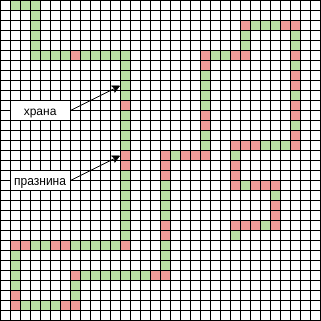
\includegraphics[scale=0.30]{santa_fe.png}
    \end{minipage}
\end{frame}

\subsection[Медицина и економија]{Медицина и економија}

\begin{frame}{Примери примене и мета-генетичко програмирање}
    Медицина:
    \begin{itemize}
        \item додатан аналитички алат
        \item истраживање болести попут рака
        \item класификација медицинских података коришћењем ГП-а се показало боље од класичних алгоритама машинског учења
    \end{itemize}
    Економија:
    \begin{itemize}
        \item проблем класификације код предвиђања банкрота предузећа
        \item максимизовање профита на тржиштима хартија од вредности
    \end{itemize}
\end{frame}

\subsection[Мета-генетичко програмирање]{Мета-генетичко програмирање}

\begin{frame}{Мета-генетичко програмирање}
    \begin{itemize}
        \item Упоредно еволуирање програма који врши генетичко програмирање
        \item Једна од метода МГП је еволуирање оператора мутације
        \begin{itemize}
            \item Јединке су оператори мутације приказани помоћу синтаксних стабла
            \item Оператори садрже кораке који мењају гене над којима се врши мутација
            \end{itemize}
        \item Прилагођеност јединке се мери кроз прилагођеност јединки које генерише
        \item Изискују више рачунарских ресурса
    \end{itemize}
\end{frame}
    
\begin{frame}{Мета-генетичко програмирање}
    \begin{figure}
        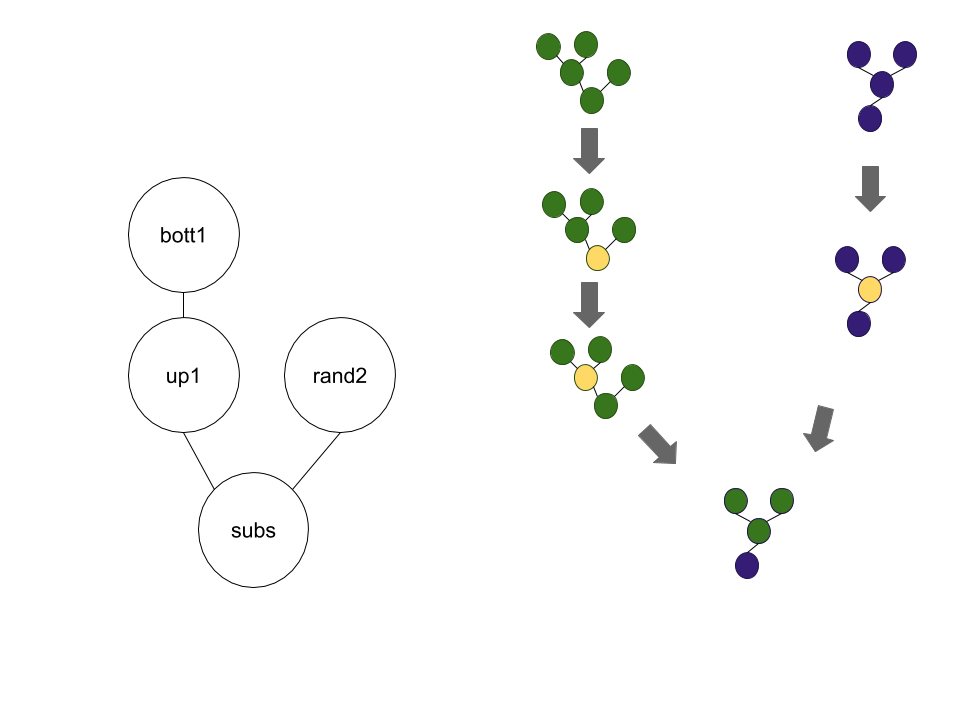
\includegraphics[scale=0.3]{mgp_primer.png}
    \end{figure}
\end{frame}

\appendix

\renewcommand\refname{Литература}

\begin{frame}{Литература}
    \nocite{*}
    \printbibliography
\end{frame}


\section{}
\begin{frame}{}
    \centering
    \Huge\bfseries{Хвала на пажњи!\\ Питања?}
\end{frame}

\end{document}
